%=======================+=========================
%==============  Trigger    ================
%=================================================\

\section[Trigger]{Trigger \label{sec:trig}}
The goal of the \gx{} trigger is to accept most high-energy hadronic interactions while reducing the background rate induced by electromagnetic and low-energy hadronic interactions to the level acceptable 
by the data acquisition system (DAQ).  The main trigger algorithm is based on measurements of energy depositions in the FCAL and BCAL as described in Ref.~\cite{somov_l1,somov_l11}. Supplementary triggers can also use hits from scintillator detectors, such as the PS, tagging detectors, ST, TOF, and TAC.

\subsection{Architecture \label{sec:trigarchitecture}}
The \gx{} trigger system\cite{GlueX:2013twa} is implemented on dedicated programmable pipelined electronics modules, designed at JLab using Field-Programmable Gate Arrays (FPGAs).  The \gx{} trigger and readout electronics are hosted in VXS (ANSI/VITA 41.0) crates. VXS is an extension of the VME/VME64x architecture, which uses high-speed backplane lines to transmit trigger information. 

A layout of the trigger system is presented in Fig.~\ref{fig:trig}. Data from the FCAL and BCAL are sent to  FADC modules~\cite{Dong:2007}, situated in 12 and 8 VXS crates, respectively, and are digitized at the sampling rate of 250 MHz. The digitized amplitudes are used for the trigger and are also stored in the FPGA-based pipeline for subsequent readout via VME.
Digitized amplitudes are summed for all 16 FADC250 channels in each 4 ns sampling interval and are transmitted to the crate trigger processor (CTP) module, which sums up amplitudes from all FADC boards in the crate. The sub-system processor (SSP) modules located in the global trigger crate receive amplitudes from all crates and compute the total energy deposited in the FCAL and BCAL. The global trigger processor (GTP) module collects data from the SSPs and makes a trigger decision based on the encoded trigger equations. The core of the trigger system is the trigger supervisor (TS) module, which receives the trigger information from the GTP and distributes triggers to the electronics modules in all readout 
crates in order to initiate the data readout. The \gx{} system has 55 VXS crates in total (26 with FADC250s, 14 with  FADC125s, 14 with F1 TDCs, and 1 CAEN TDC). The TS also provides a synchronization of all crates and provides a 250 MHz clock signal. The triggers and clock are distributed through the trigger distribution (TD) module in the trigger distribution crate. The signals are received by the trigger interface (TI) module and signal distribution (SD) module in each crate. The \gx{} trigger system provides a fixed latency. The longest trigger distribution time of about 3.3 $\mu$s is due to the distance of the tagger hall from Hall D.
The smallest rewritable readout buffer, where hits from the detector are stored, corresponds to about 3.7~$\mu$s for the F1 TDC module. The trigger jitter does not exceed 4 ns.


\begin{figure}[tbp]
\begin{center}
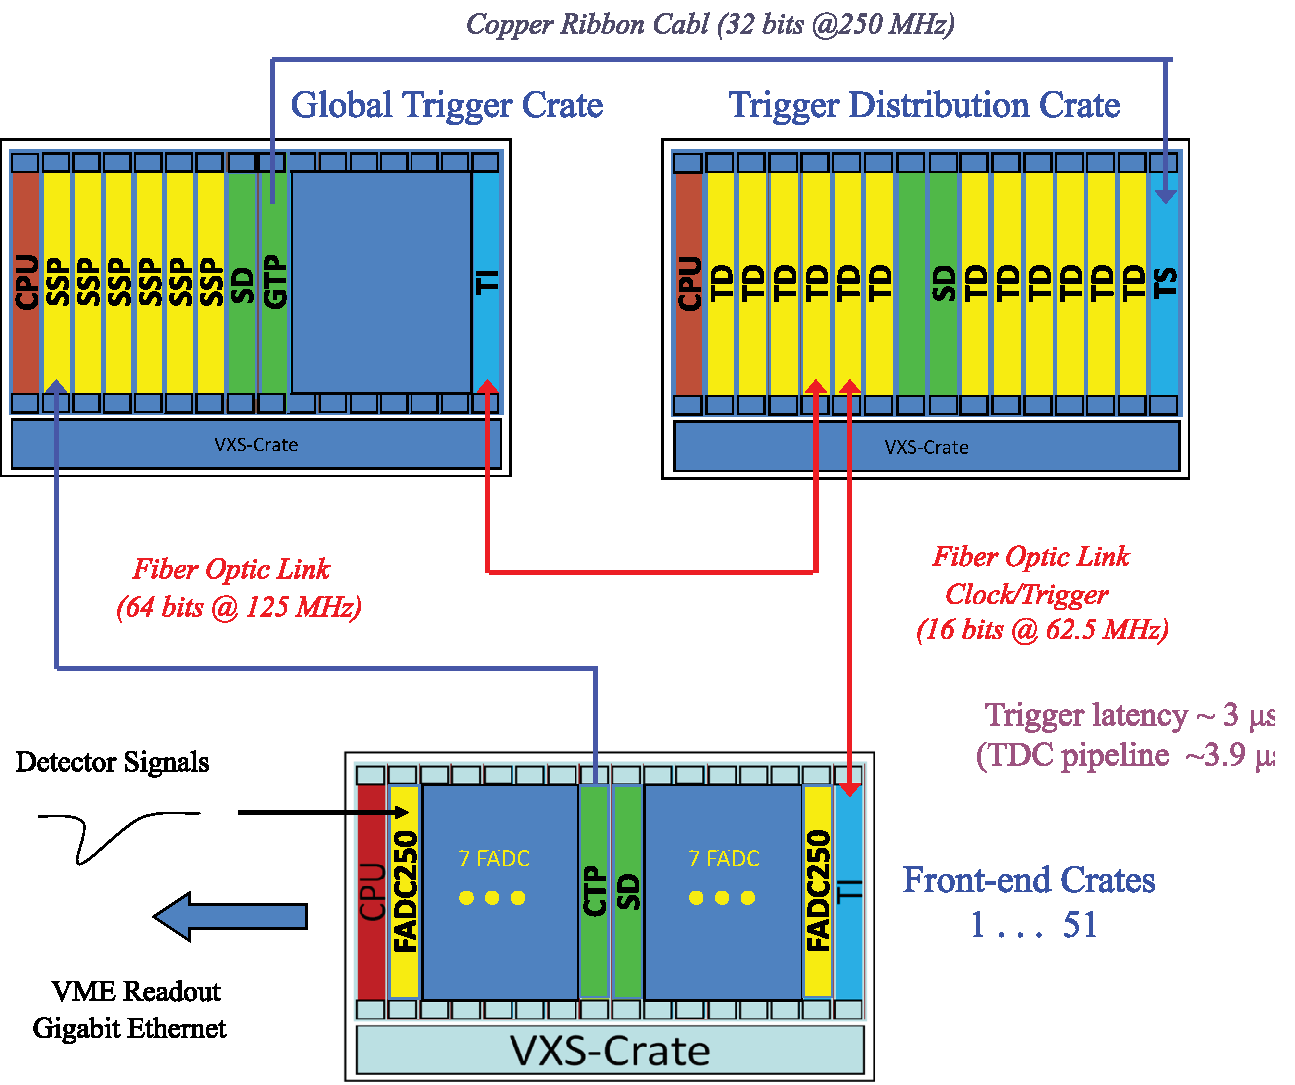
\includegraphics[width=0.75\textwidth]{figures/125_Somov-f1.pdf}  
\caption{Schematic view of the Level-1 trigger system of the \gx{} experiment. The electronics boards are described in the text.} \label{fig:trig}
\end{center}
\end{figure}

\subsection{Trigger types \label{sec:triggers}}

The \gx{} experiment uses two main trigger types: the pair spectrometer trigger, and the physics trigger based on energy depositions in the BCAL and FCAL. The 
pair spectrometer trigger is used to measure the flux of beam photons. This trigger requires a time coincidence of hits in the 
two arms of the PS detector, described in Section~\ref{sec:ps}. The physics triggers are generated when the FCAL and BCAL energies  satisfy the following conditions: 
\begin{enumerate}
\item $2\cdot E_{\rm FCAL} + E_{\rm BCAL}  > 1\;{\rm GeV},  E_{\rm FCAL} > 0\; {\rm GeV}$, \rm{and}  \\
\item $E_{\rm BCAL}  >  1.2\;{\rm GeV}$.
\end{enumerate}
The first condition defines the main trigger that uses the fact that most events produce forward-going energy. The second trigger type is used to accept events with large transverse energy released in the BCAL, such as decays of $J/\psi$ mesons. 

Several other trigger types were implemented for efficiency studies and detector calibration. 
Efficiency of the main production trigger was studied using a trigger based on the coincidence of hits from the ST and TAGH, detectors not used in the main production trigger. A combination of the PS and TAC triggers was used for the acceptance calibration of the PS, described in Section~\ref{sec:ps_flux}. Ancillary minimum-bias random trigger and calorimeter LED triggers were collected concurrently with data taking.

\subsection{Performance \label{sec:trigperformance}}
The rate of the main physics triggers as a function of the PS trigger rate is shown in Fig.~\ref{fig:trig_rate}.
The typical rate of the PS trigger in spring 2018 was about 3~kHz, which corresponds to a photon beam flux of $2.5\cdot 10^7\; \gamma/{\rm sec}$ in the coherent peak range. The total trigger rate was about 40 kHz. The rates of the random trigger and each of the LED calorimeter triggers were set to 100 Hz and 10 Hz, respectively. The electronics and DAQ were running with a livetime close to 
$100 \%$, collecting data at a rate of 600 MB per second.
The trigger system can operate at significantly higher rates, considered for the next phase
of the GlueX experiment. The combined dead time of the trigger and DAQ systems at the trigger rate of 80 kHz
was measured to be about $10 \%$. The largest contribution to the dead time comes from the hit processing
time of readout electronics modules. 

%In spring 2018, data were collected at the luminosity %corresponding to the photon beam flux of about $2.5\cdot 10^7\; %\gamma/{\rm sec}$ in the GlueX energy range of interest. The %typical rate of the PS trigger 

\begin{figure}[tbp]
\begin{center}
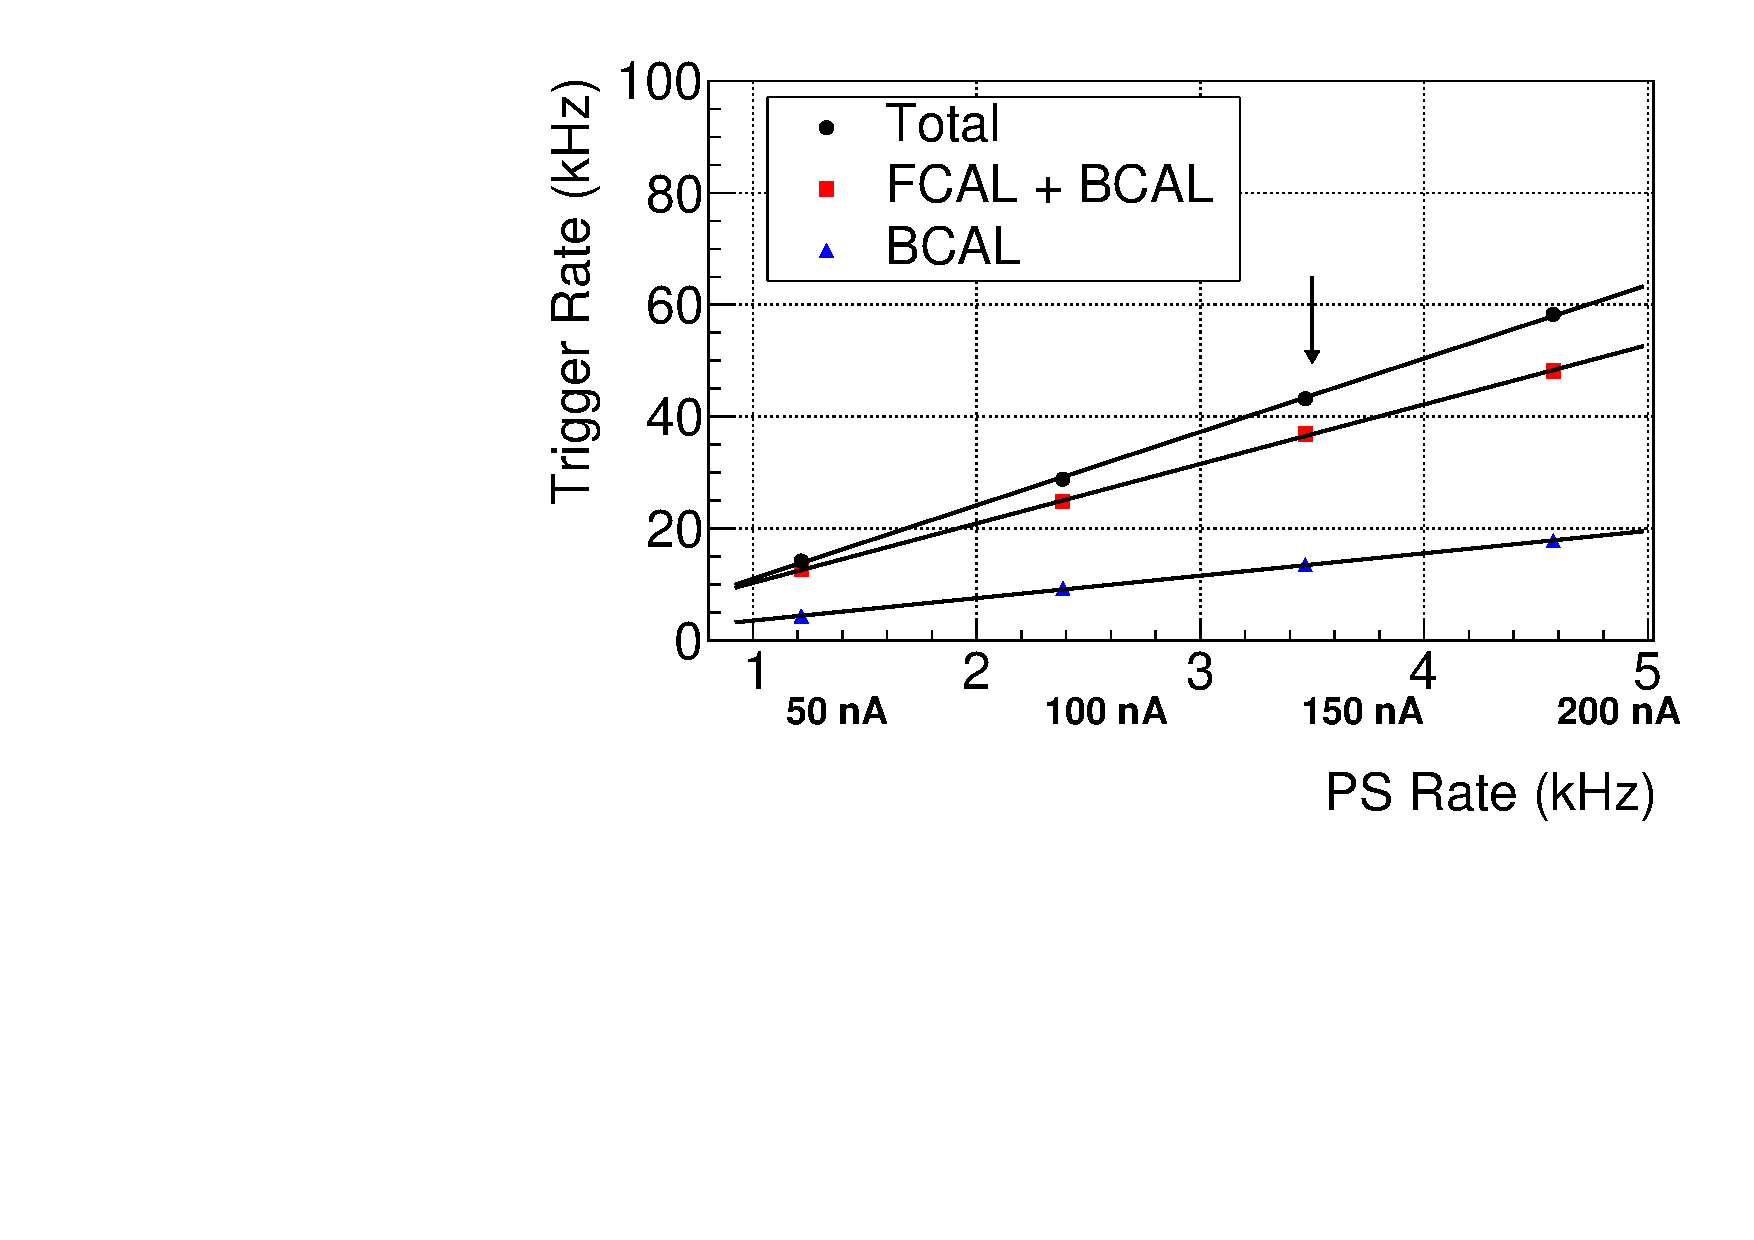
\includegraphics[width=0.5\textwidth]{figures/plot_triggerL1_c1}  
\caption{Rates of the main production triggers as a function of the PS rate: FCAL and BCAL trigger (boxes), BCAL trigger (triangles), the total trigger rate (circles). The vertical arrow indicates the run conditions during the spring of 2018 with a diamond
radiator, 5 mm collimator and 75 $\mu$m Be converter.} \label{fig:trig_rate}
\end{center}
\end{figure}
